\section{Búsqueda de contratos inteligentes similares}
\label{appendix:sim_code}

La dificultad en la búsqueda de similaridad de código radica en las características estructurales de los lenguajes de alto nivel, y en la diversidad de las expresiones lógicas de los contratos inteligentes. En la actualidad existen varias escuelas de algoritmos de búsqueda de similaridad de código en los círculos académicos, las que se describen de este modo:

\begin{itemize}
	\item \textbf{Distancia de edición entre cadenas de caracteres} \\
	Tanto la consulta de código como el código fuente candidato se consideran como texto. La distancia de edición entre dos cadenas de caracteres se utiliza para medir las similitudes entre ambos. La \textit{distancia de edición} se refiere al número mínimo ded operaciones de edición necesarias para convertir una cadena de caracteres en otra. Las operaciones de edición permitidas incluyen la sustitución de un carácter por otro —borrado de un carácter e inserción de otro—. Generalmente hablando, a menor distancia de edición, mayor la similitud entre dos cadenas de caracteres. Este algoritmo basado en distancias de edición entre cadenas de caracteres puede ser usado no sólo para la comparación de códigos fuente sino también en representaciones intermedias o incluso código de máquina.
	Con el fin de mejorar la robustez de estos algoritmos, se llevará a cabo un cierto grado de conversión del código fuente sin introducir cambios semánticos: esto puede ser la remoción de caracteres en blanco, la remoción de comentarios, el reemplazo de los nombres de todas las variables locales con ‘\$’, la normalización de las expresiones algebraicas, etcétera. Este tipo de algoritmos se caracterizan por ser veloces, concisos y muy eficientes. No obstante, su adaptabilidad a programas complejos es relativamente pobre y no tienen en cuenta la sintaxis y la estructura organizativa del código.

	\item \textbf{Secuencia de tokens} \\
	El método de representación de secuencias de tokens se refiere a la conversión del código fuente ingresado en una secuencia de tokens a través del análisis léxico. La similitud entre dos programas se puede ver como la similitud entre dos secuencias de tokens, de modo que se puede utilizar la mayor subcadena en común o un algoritmo de coincidencia de correlación (algoritmo de coincidencia de árboles de sufijos) para medir el grado de similitud entre dos programas, a través del cual se pueden detectar segmentos de código con diferentes sintaxis pero con funciones similares. Sin embargo, este método oculta la estructura organizativa de los programas al medir la similitud entre ellos.

	\item \textbf{Árbol de sintaxis abstracta (\textit{Abstract Syntax Tree}, o AST)} \\
	AST es una forma de expresión intermedia después de realizar un análisis sintáctico en un código fuente, sobre el cual se puede medir la similitud entre dos programas a través de la comparación entre un subárbol y otro. Para medir la similitud entre dos árboles se puede utilizar el algoritmo de distancia de edición de árbol \cite{zhang1989simple}. El algoritmo preciso de la distancia de edición del árbol es relativamente complejo y la literatura al respecto (\cite{guha2002approximate}) proporciona un algoritmo rápido aproximado. De acuerdo a \cite{chilowicz2009syntax}, los árboles de sintaxis deben someterse a una identificación por huella hash con el fin de habilitar al algoritmo de comparación del árbol de sintaxis para realizar búsquedas de alta eficiencia en conjuntos de datos masivos.

	\item \textbf{Grafo de dependencias de programas (\textit{Program Dependency Graph}, o PDG)} \\
	Un PDG \cite{ferrante1987program} puede representar los datos internos, controlar la relación de dependencia de un programa y analizar el código de programa a nivel semántico. Un protocolo de código similar se transforma en una búsqueda de subgrafos isomórficos, que es un problema NP-completo y requiere un algoritmo muy complejo, por lo que sólo algunos algoritmos aproximados están disponibles en la actualidad.

\end{itemize}

Creemos que los algoritmos mencionados describen las similitudes entre códigos en texto, estructura y sintaxis en dimensiones diferentes. Source Forager \cite{kashyap2017source} nos proporciona un gran ejercicio mental: los índices de similitud en distintas dimensiones se representan como características diferentes, cada una de las cuales representa la medición de la similitud del código desde un aspecto específico. Por último, la similitud vectorial se utiliza para llevar a cabo la medición de la similitud general. Este método integra las ventajas de los algoritmos mencionados anteriormente. Esta idea también es utilizada por Nebulas como referencia para realizar la búsqueda de la similitud entre contratos inteligentes. Consideramos que funciona como la unidad fundamental de búsqueda de código entre los contratos inteligentes.

La tabla \ref{table:search-similarity} define las características de similitud entre códigos candidatos. Luego, se describe la definición de cada característica y la función para calcular su similitud:

\begin{table}[h]
\centering
\begin{threeparttable}[b]
\caption{Tabla de familias de características de similitud de código}
\label{table:search-similarity}
\begin{tabular}{ccc} \toprule
    {Clase de características} & {Descripción} \\ \midrule
Emparejamiento tipo-operación & Tipos empleados y operaciones realizadas sobre esos tipos \\
Esqueleto de árbol & Estructura de bucles y condicionales \\
Esqueleto de árbol decorado & Estructura de bucles, condicionales y operaciones \\
BFS sobre 3-grafo del CFG & Subgrafos de un CFG de tamaño 3, usando BFS para generar subgrafos \\
BFS sobre 4-grafo del CFG & Subgrafos de un CFG de tamaño 4, usando BFS para generar subgrafos \\
DFS sobre 3-grafo del CFG & Subgrafos de un CFG de tamaño 3, usando DFS para generar subgrafos \\
DFS sobre 4-grafo del CFG & Subgrafos de un CFG de tamaño 4, usando DFS para generar subgrafos \\
Llamadas a librerías & Llamadas a librerías \\
Signatura & Tipos de entrada y valor devuelto \\
Tipos locales & Tipos de las variables locales \\
Literales numéricos & Constantes de datos numéricos \\
Literal de cadena & Constantes de datos de cadena \\
\bottomrule
\end{tabular}
\end{threeparttable}
\end{table}

\begin{itemize}
	\item \textbf{\textit{Emparejamiento tipo-operación}} \\
	Es un conjunto 2-tupla que contiene el tipo de la variable y su operador, es decir, el par (tipo, operación). Generalmente, los tipos de datos primitivos debe emparejarse con un operador aritmético, un operador lógico y un operador relacional, tal como ($int, \geq$); los tipos de datos personalizados (como las estructuras \texttt{struct}) deben emparejarse con las funciones miembro, tales como (\texttt{Bar}, \texttt{.foo}), indicando que el campo \texttt{foo} del tipo de dato \texttt{Bar} es consultado. Basándonos en esta metodología, todas las operaciones sobre variables en el cuerpo del código de una función se deben transformar en 2-tuplas.

	Después de eliminar repeticiones, se utiliza una secuencia 2-tupla para reflejar la característica de emparejamiento tipo-operación de este segmento de código. Creemos que las piezas de código con funciones similares deben tener similares conjuntos de operaciones sobre variables. No obstante, no nos preocupa el orden de las 2-tuplas, por lo que esta característica pierde la información de la estructura lógica del código y por lo tanto sólo puede representar parcialmente sus características.

	La similitud entre las características de emparejamiento tipo-operación se puede definir mediante similitudes Jacobianas; es decir que dados dos conjuntos $S_1$ y $S_2$, la similitud Jacobiana se puede definir mediante la siguiente fórmula:

	\begin{equation}
	sim_{Jacc(S_{1}, S_{2})}=\frac{\mid S_{1}\bigcap S_{2}\mid}{\mid S_{1}\bigcup S_{2}\mid}
	\end{equation}

	\item Esqueleto de árbol (\textit{Skeleton Tree}) \\
	Árbol de sintaxis abstracta basado en código. Sólo se mantienen las estructuras de bucle (\texttt{for, while, do...while}) y las sentencias condicionales (\texttt{if...else}); todos los otros nodos son removidos del árbol. Creemos que los códigos con funciones similares deberían ser similares en cuanto a estructuras de bucle y sentencias condicionales.

	El cálculo de la similitud para esqueletos de árbol está basado en la distancia de edición entre dos árboles. Se define $d_{r}$ como la distancia de edición estimada entre dos árboles, y está determinada únicamente por el tamaño del árbol, es decir:

	\begin{equation}
	d_{r}(T_{1}, T{2})=\frac{\mid size(T_{1})-size(T_{2})\mid}{max(size(T_{1}), size(T_{2}))}
	\end{equation}

	Se asume $D_T$ como el valor umbral de la distancia de edición, y se fija en 0,5. Podemos adquirir la fórmula para el cálculo de la distancia aproximada de edición entre dos árboles:

	\begin{equation}
	d_{t}(T_{1}, T{2})=\begin{cases}d_{r}(T_{1}, T{2}) & if~d_{r}(T_{1}, T{2})\geq D_{T}\\\frac{max\left(\begin{array}{c}ed(pre(T_{1}),~pre(T_{2})),\\ ed(post(T_{1}),~post(T_{2}))\end{array}\right)}{max(size(T_{1}), size(T_{2}))} & otherwise\end{cases}
	\end{equation}

	$pre(T)$ representa la secuencia transversal del árbol antes de la ordenación; $post(T)$ representa la secuencia transversal del árbol después de la ordenación; $ed(S_{1}, S_{2})$ representa la distancia de edición entre $S_{1}$ y $S_{2}$. La similitud entre dos esqueletos de árbol se puede calcular mediante la siguiente fórmula:

	\begin{equation}
	sim_{Tree}(T_{1}, T{2})=1-d_{t}(T_{1}, T{2})
	\end{equation}

	\item Esqueleto de árbol decorado (\textit{Decorated Skeleton Tree}) \\
	Esta entidad es similar al esqueleto de árbol, aunque además de preservar los nodos de bucle y bifurcación, se conservan la mayoría de los operadores (tales como \texttt{+, -, <}), excepto por \texttt{=} y \texttt{\&}, considerados como \textit{ruido}.

	\item \textbf{K-subgrafos del CFG} \\
	Dado un CFG\footnote{CFG aquí refiere a la locución inglesa \textit{Control Flow Graph}, es decir, grafo de flujo de control (N. del T.)} y un nodo específico, se lleva a cabo una búsqueda BFS\footnote{\textit{Breadth-First Search}, o \textit{búsqueda en anchura} (N. del T.)} o bien una búsqueda DFS\footnote{\textit{Depth-First Search}, o \textit{búsqueda en profundidad} (N. del T.)} hasta que el número de nodos recorridos llegue a $k$, momento en el cual el subgrafo formado debería ser el k-subgrafo. Si el número de nodos no llega a $k$ luego de finalizar el recorrido, dicho subgrafo se debe descartar. Mediante el recorrido de cada nodo en el CFG, podemos adquirir todos los k-subgrafos. Por cada k-subgrafo, es necesario utilizar un entero de $k^2$ bits para expresarlo. Para más detalles, consúltese la \ref{fig:graph-ex}. Todos los k-subgrafos forman un conjunto de enteros.

	\textbf{BFS sobre 3-grafo del CFG:} k = 3, recorrido de árbol BFS

	\textbf{BFS sobre 4-grafo del CFG:} k = 4, recorrido de árbol BFS

	\textbf{DFS sobre 3-grafo del CFG:} k = 3, recorrido de árbol DFS

	\textbf{DFS sobre 4-grafo del CFG:} k = 4, recorrido de árbol DFS

	Dados los vectores $\vec{x}=(x_{1}, x_{2}, ...x_{n})$ y $\vec{y}=(y_{1}, y_{2}, ...y_{n})$, la similitud Jacobiana generalizada se puede definir como:

	\begin{equation}
	J(\vec{x}, \vec{y})=\frac{\sum_imin(x_{i}, y_{i})}{\sum_imax(x_{i}, y_{i})}
	\end{equation}

	\begin{figure}[h]
	\centering
	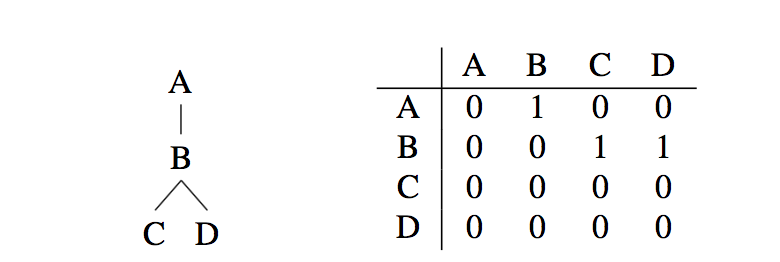
\includegraphics[width=6cm]{./figs/graph-matrix.png}
	\caption{Ejemplo para un 4-grafo: el elemento de la matriz es la cadena binaria \texttt{0100 0011 0000 0000}, que representa el número decimal es 17 152}
	\label{fig:graph-ex}
	\end{figure}

	\item \textbf{Llamadas a librerías} \\
	Si dentro del contrato se realiza una llamada a un contrato-librería, se registrarán las direcciones de todos los contratos-librería, y la similitud se calculará mediante la fórmula de similitud Jacobiana.

	\item \textbf{Signatura} \\
	Consiste en registrar el tipo de los parámetros y el tipo del valor de retorno de la función; la similitud se calcula mediante la fórmula de similitud Jacobiana. Por ejemplo, para el siguiente código de un contrato inteligente, la característica \textit{signatura} de la función \texttt{getBalance} es el vector \texttt{(address, uint256)}. \\

	\begin{figure}[h]
  	\centering
  	\begin{minipage}{.7\linewidth}
	\begin{lstlisting}[frame=single]
contract addressTest {
  function getBalance(address addr) returns (uint) {
  	return addr.balance;
  }
}
	\end{lstlisting}
  	\end{minipage}
	\end{figure}

	\item \textbf{Tipos locales:} esta característica es el conjunto de todos los tipos de las variables locales de la función \texttt{body}, para el que debe calcularse la similitud mediante la fórmula de similitud Jacobiana.

	\item \textbf{Literales numéricos:} el conjunto de todas las constantes numéricas sirve como la característica de los \textit{literales numéricos}, para el que debe calcularse la similitud mediante la fórmula de similitud Jacobiana.

	\item \textbf{Literales de cadena:} el conjunto de todas las constantes de cadena sirve como la característica de los \textit{literales de cadena}, para el que debe calcularse la similitud mediante la fórmula de similitud Jacobiana.
\end{itemize}

La familia de características se puede expandir, por lo que es conveniente añadir nuevas características a ella. Basándonos en la circunstancia de que existe un cálculo de similitud por cada característica, podemos calcular la suma ponderada de todas las características y así adquirir la similitud final del código:

\begin{equation}
	sim_{combined}(\vec{A}, \vec{B})=\frac{\sum_{c=1}^{n_{cl}}sim_{c}(\vec{A_c},~\vec{B_c})\cdot w_{c}}{\sum_{c=1}^{n_{cl}}w_{c}}
\end{equation}

En donde $\vec{A}$ y $\vec{B}$ son vectores propios; $n_{cl}$ es el número de características en la familia; $sim_{c}$ es la función de cálculo de similitud específica de la característica c; $\vec{A_c}$ y $\vec{B_c}$ son vectores propios de la característica c; $w_{c}$ es la ponderación de c. La ponderación se puede hallar mediante el entrenamiento de algoritmos de aprendizaje de máquinas basado en un gran número de equipos de prueba.